\chapter{Conception fonctionnelle et technique}
\vspace{-1.5em}
\chaptertoc
\vspace{-2.5em}
\section{Introduction}

Ce chapitre décrit les étapes de la conception fonctionnelle et technique de la solution. Il couvre l’analyse des besoins, qu’ils soient fonctionnels ou non fonctionnels, l’étude de l’existant, l’architecture technique, ainsi que les technologies choisies pour le développement du système.

\vspace{-1.2em}
\section{Analyse des besoins}

Cette section identifie les besoins en distinguant les exigences fonctionnelles (comportements attendus) des non fonctionnelles (performances requises).
\vspace{-1.2em}
\subsection{Processus d’identification des besoins}
L’identification des besoins, menée par le Product Owner lors d’ateliers métier, a permis de préciser les attentes fonctionnelles, techniques et les enjeux opérationnels.

Un membre de notre équipe a assisté à une réunion sur site à l’\ac{ONDA}, facilitant l’analyse des données et les échanges avec les équipes.

Des discussions en ligne avec la DSI ont complété ce travail en clarifiant les aspects techniques et les besoins liés à l’exploitation et la qualité des données.
\vspace{-1.2em}

\subsection{Les besoins fonctionnels}

Le système doit permettre l’\textbf{ingestion, le traitement et la validation de données} issues de diverses sources (AODB, COSMOS, SMART\footnote{SMART : plateforme de supervision opérationnelle et de reporting temps réel}, SMART, Excel, API), avant leur stockage dans un datalake.

Il doit assurer une \textbf{planification intelligente des stands}, en prédisant les affectations optimales selon plusieurs critères (type d’avion, vol, occupation...), avec possibilité de comparaison à la planification actuelle (\ac{SOAM}) et d’ajustements manuels.

La solution proposera des outils de \textbf{simulation et d’aide à la décision} : simulation d’activité, visualisation via jumeau numérique et indicateurs clés (OTP, retards...).

Des \textbf{interfaces intuitives} sont attendues pour visualiser les plannings, configurer les objectifs et faciliter la coordination (chat, appels...).

Enfin, le système devra générer des \textbf{alertes personnalisables} en cas d’anomalies, et offrir une \textbf{recherche rapide} pour localiser un avion ou un stand.

\subsection{Besoins non fonctionnels}
\vspace{-0.5em}
Le système doit garantir la \textbf{sécurité et la gouvernance des données} (authentification, autorisation, chiffrement, traçabilité et gestion du cycle de vie).

Il doit être \textbf{scalable et compatible avec le Cloud}, via une architecture modulaire et une intégration avec des plateformes comme Cloudera.

La \textbf{surveillance et l’automatisation} sont également clés : supervision proactive des flux critiques et automatisation des services sensibles.

L’\textbf{interopérabilité} avec les systèmes \ac{ONDA} existants est requise, assurant des échanges fluides entre Cloudera et les bases métier.

Enfin, la \textbf{gestion des risques} implique l’identification des menaces potentielles et la mise en œuvre de plans de contingence adaptés.

\vspace{-1.2em}

\section{Analyse de l’existant}

Avant de proposer une solution d’optimisation, il est essentiel d’analyser l’existant afin d’identifier les forces et les limites du système actuellement en place.
\vspace{-1.2em}
\subsection{Étude de l'existant}

\noindent
Le Système d'Optimisation et d'Affectation des Moyens (\ac{SOAM}) s’inscrit dans la feuille de route 2018–2025 de modernisation de l’\ac{ONDA}. Il a pour vocation de centraliser et automatiser la planification des ressources aéroportuaires dans 22 aéroports marocains.  

\vspace{0.6em}  

\textbf{Planification saisonnière.} Les compagnies aériennes transmettent leurs plannings (été/hiver) au coordinateur marocain des créneaux horaires aériens (MSC)\footnote{MSC : \textit{Moroccan Slot Coordinator}} sous format Excel. Ces fichiers sont ensuite transférés manuellement à la cellule de planification des vols (CPV)\footnote{CPV : Cellule de Planification des Vols}.  

\vspace{0.6em}  

\textbf{Intégration dans SOAM.} Les données sont vérifiées et converties manuellement au format CSV. Le chargement dans le système doit être fait cinq jours avant le début de la saison. Aucun mécanisme de validation automatique n’est mis en place, exposant à des erreurs de saisie.   

\vspace{0.6em}  

\textbf{Gestion des modifications.} Les mises à jour des vols (horaires, annulations...) sont reçues soit via \textbf{SITA} (intégration automatique), soit via \textbf{Outlook} (traitement manuel par la cellule PCO\footnote{PCO : \textit{Poste de Coordination Opérationnelle}}).  

\vspace{0.6em}  

\textbf{Visualisation des stands.} Une interface graphique (Figure~\ref{fig:graphiqueSOAM}) permet de visualiser les avions affectés aux stands sur le plan de l’aéroport. Cette vue facilite la coordination opérationnelle en montrant la position physique des aéronefs, les zones de sécurité, et les services de piste.

\begin{figure}[H]
	\centering
	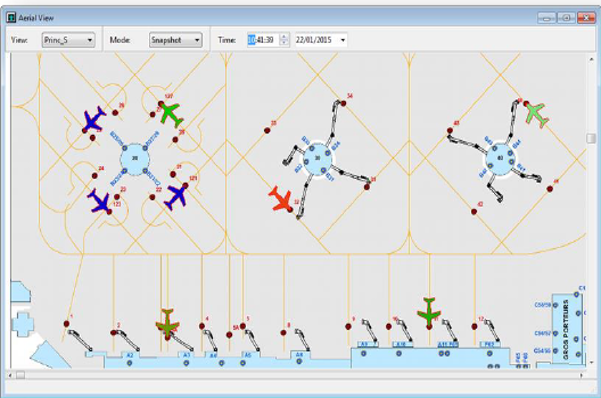
\includegraphics[width=0.5\textwidth]{assets/diagrams/graphiqueSOAM.png}
	\caption{Vue graphique de la planification des stands sur le plan de l'aéroport}
	\label{fig:graphiqueSOAM}
\end{figure}
\vspace{-1.2em}
\textbf{Mécanisme de planification.} \ac{SOAM} repose sur un ensemble de règles prédéfinies pour générer une planification initiale, qui peut être manuellement ajustée en cas de conflit. Aucune logique d’optimisation ni moteur d’aide à la décision n’est actuellement intégré.

\subsection{Identification des limitations de l'existant }

Le système actuel présente quatre principales limites :  

\begin{enumerate}
	\item \textbf{Processus inefficaces} : forte dépendance aux interventions manuelles, avec des délais importants entre réception et intégration des plannings.  
	\item \textbf{Manque d’intelligence} : absence d’IA, sans recommandations ni simulations, fonctionnement basé sur des règles statiques sans adaptation dynamique.  
	\item \textbf{Fonctionnalités limitées} : interfaces peu ergonomiques, pas de visualisation 3D ni collaboration intégrée, absence d’indicateurs avancés (KPI).  
	\item \textbf{Impact sur la performance} : sous-utilisation des ressources, mauvaise gestion des crises, expérience utilisateur dégradée (lenteur, difficulté d’apprentissage).
\end{enumerate}

En résumé, le \ac{SOAM} répond aux besoins de base, mais reste limité en résilience et optimisation. Une plateforme intelligente, modulaire, connectée, intégrant un \textit{data lake}, l’IA et un jumeau numérique, s’impose.


\vspace{-1.2em}




\section{Architecture technique}

Cette section présente la structure technique sur laquelle repose la solution proposée, en mettant en avant ses composants clés et l'architecture d'intelligence artificielle

\subsection{Vue d'ensemble}

La modernisation des opérations aéroportuaires vise plusieurs objectifs interdépendants : optimiser les flux passagers, améliorer la gestion des bagages, coordonner les rotations avion, anticiper les capacités et planifier intelligemment les stands. Ces fonctions nécessitent une infrastructure unifiée capable de traiter des données hétérogènes en temps quasi réel.

La planification des stands joue un rôle central dans cette chaîne. Elle impacte directement la ponctualité, l’occupation des ressources au sol et la fluidité globale des opérations. La solution proposée s’appuie sur une architecture modulaire et scalable, intégrant les technologies Big Data et l’IA pour analyser les données issues de multiples sources (\ac{AODB}, météo, mouvements avion...).


\begin{figure}[H]
	\centering
	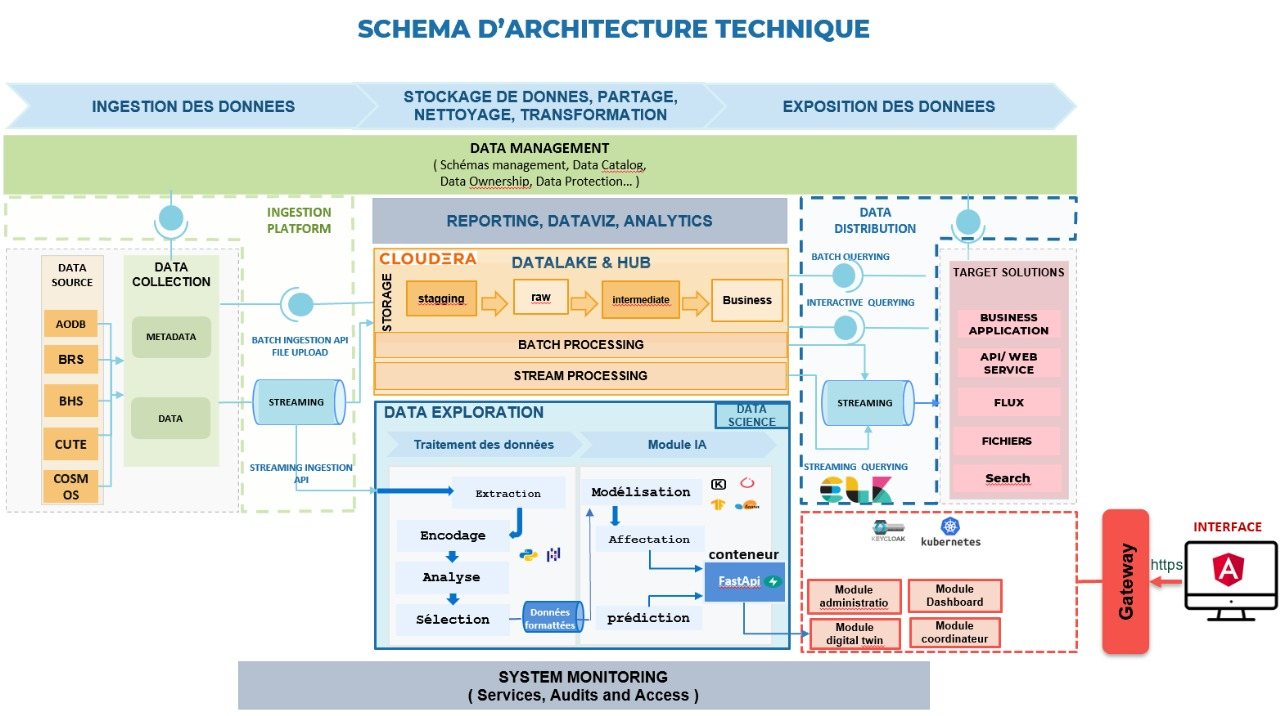
\includegraphics[width=1.1\linewidth]{assets/architecture/architecture.jpg}
	\caption{Architecture globale de la solution intelligente de la planification des stands}
	\label{fig:architecture}
\end{figure}

L’architecture se compose des éléments suivants :

\begin{itemize}
	\item \textbf{Sources de données} : les données sont collectées en temps quasi réel à partir de systèmes existants comme \ac{AODB}, COSMOS\footnote{COSMOS : système de gestion technique et logistique des infrastructures aéroportuaires}, fichiers Excel, API et autres bases relationnelles.
	
	
	\item \textbf{Ingestion et traitement des données} : un pipeline d’ingestion automatisé alimente un \textbf{Data Lake} hébergé sur une plateforme Big Data \textbf{(Cloudera)}, en assurant le nettoyage, la normalisation et la transformation des données.
	
	\item \textbf{Stockage centralisé} : les données sont stockées de manière structurée et non structurée dans le Data Lake, facilitant les accès parallèles et les traitements distribués.
	
	\item \textbf{Moteur d’intelligence artificielle} : les modèles d’optimisation (basés sur le Machine Learning et des algorithmes de recherche opérationnelle) utilisent les données historiques et en temps quasi réel pour générer des recommandations de planification.
	
	\item \textbf{Moteur de simulation} : permet de tester plusieurs scénarios de planification (ex : jour perturbé, saturation, retards massifs) et d’évaluer les impacts sur la performance.
	
	\item \textbf{Interface utilisateur} : une application graphique (vue 3D) permet aux équipes opérationnelles de consulter les recommandations, visualiser les affectations sur un plan de l’aéroport, simuler des scénarios, et interagir avec le système (modification, validation, alertes, chat).
	
	\item \textbf{Reporting et pilotage} : des tableaux de bord fournissent des indicateurs clés (KPI) tels que le taux d’occupation, l’OTP (on-time performance), le taux de replanification, ou encore les conflits évités.
\end{itemize}




Cette architecture répond aux besoins de performance, de flexibilité et d’adaptabilité d’un environnement aéroportuaire en constante évolution.



\subsection{Zoom sur l'architecture du module d’intelligence artificielle}


Le module d’intelligence artificielle constitue le cœur du système d’optimisation. Il est conçu pour automatiser et améliorer les décisions relatives à l’affectation des stands, tout en offrant une extensibilité vers d’autres cas d’usage futurs (flux passagers, rotations, bagages, capacités, etc.).

\begin{figure}[H]
	\centering
	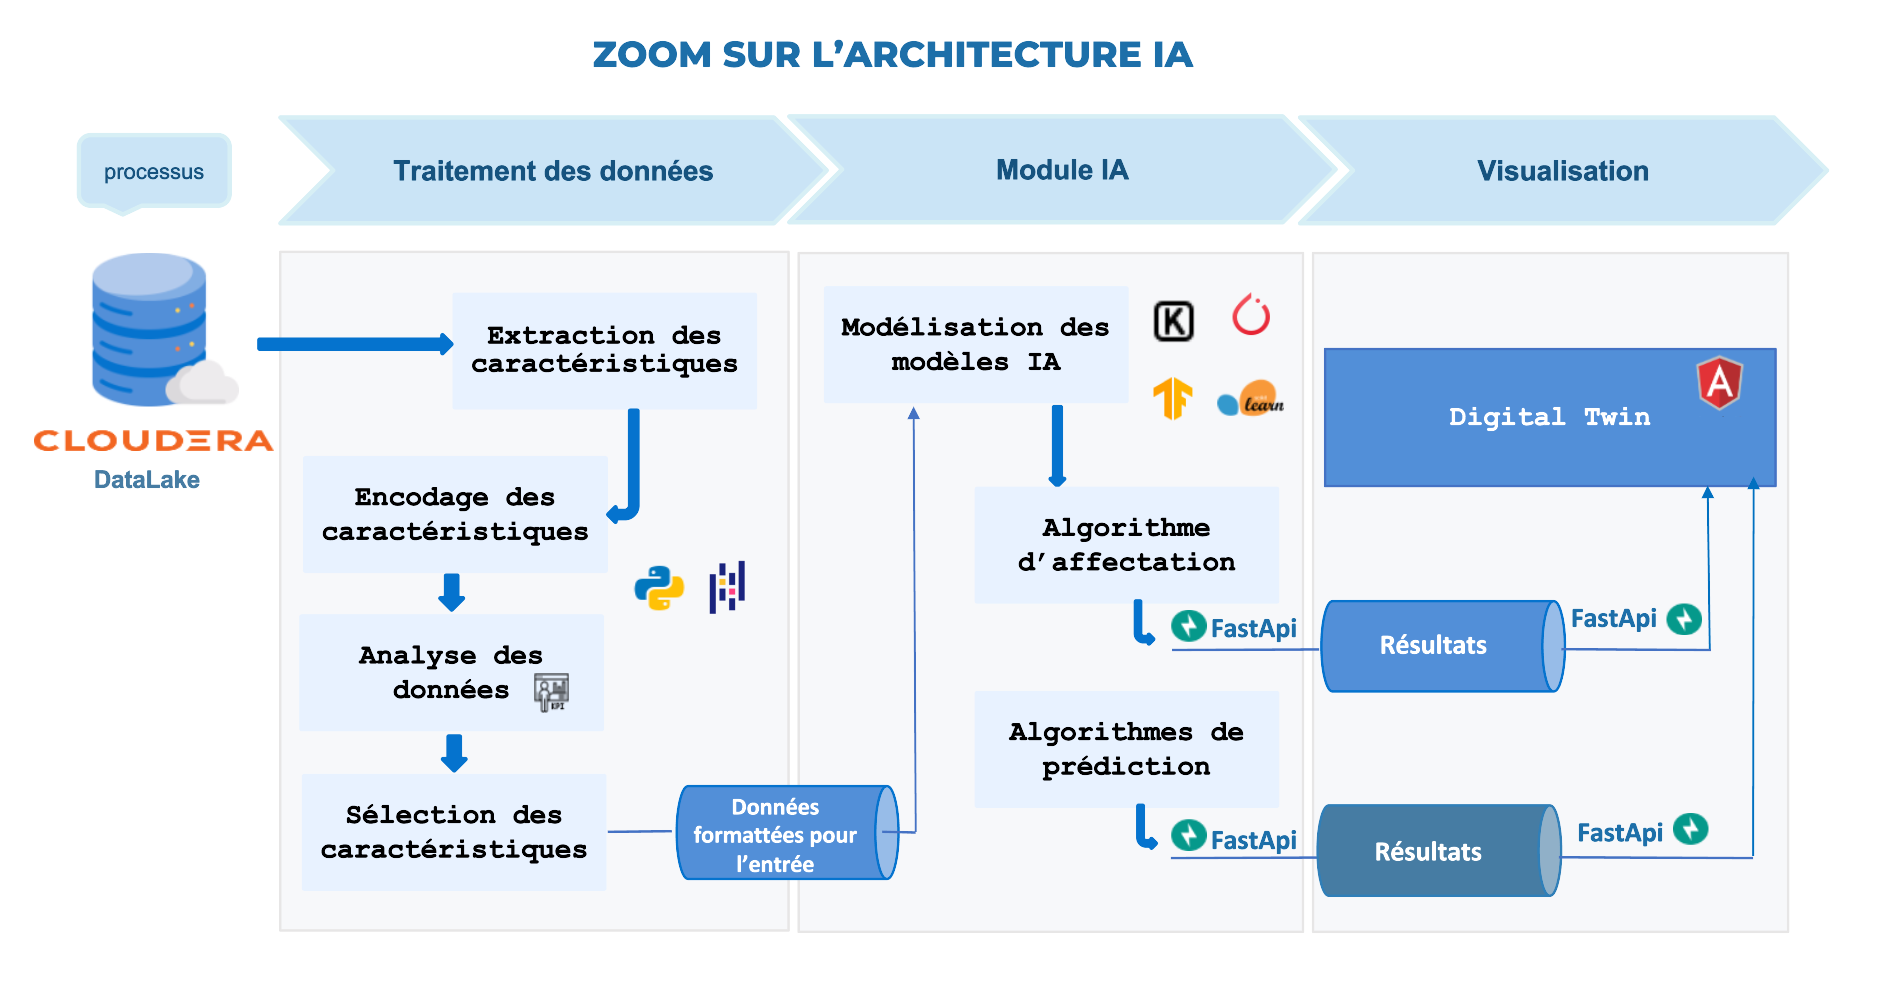
\includegraphics[width=1.1\linewidth]{assets/architecture/moduleIA.png}
	\caption{Pipeline du module IA}
	\label{fig:moduleIA}
\end{figure}


L’architecture \ref{fig:moduleIA} de ce module suit un pipeline structuré en plusieurs phases :

\begin{enumerate}
	\item \textbf{Prétraitement et préparation des données} \\[0.3em]
	Cette première étape consiste à transformer les données brutes collectées depuis les différentes sources en un format exploitable pour l’apprentissage et l’optimisation. Elle inclut :
	\begin{itemize}
		\item \textbf{Extraction des caractéristiques} : identification des variables pertinentes comme le type d’aéronef, la durée d’escale, les contraintes de compatibilité avec les stands.
		\item \textbf{Encodage des caractéristiques} : transformation des variables catégorielles (ex. type d’avion, terminal) en formats numériques utilisables par les modèles d’apprentissage.
		\item \textbf{Analyse exploratoire des données} : identification d’anomalies, visualisation des distributions, corrélations entre variables, et détection de valeurs manquantes.
		\item \textbf{Sélection des caractéristiques} : réduction de la dimensionnalité via des méthodes statistiques ou algorithmiques pour conserver les variables les plus influentes.
	\end{itemize}
	
	\item \textbf{Modélisation et optimisation IA} \\[0.3em]
	Les données préparées sont injectées dans des modèles IA en fonction du cas d’usage :
	\begin{itemize}
		\item \textbf{Algorithmes d’affectation et d’optimisation} : utilisés pour générer un planning optimisé des stands selon des contraintes d’exploitation et de compatibilité.
		\item \textbf{Modèles de prédiction et Deep Learning} : prévus pour les objectifs futurs tels que la prévision de flux passagers, la détection de saturation, ou l’anticipation de conflits.
	\end{itemize}
	
	\item \textbf{Déploiement via API et conteneurisation} \\[0.3em]
	Une fois le planning optimisé généré, les résultats sont encapsulés dans une API REST, développée avec \textbf{FastAPI}. Cette API est conteneurisée à l’aide de \textbf{Docker}.
	
	\item \textbf{Intégration applicative et visualisation} \\[0.3em]
	L’image Docker produite est transmise à l’équipe de développement pour intégration dans la plateforme. Cela permet :
	\begin{itemize}
		\item d’alimenter le \textbf{jumeau numérique} avec des scénarios réalistes de planification,
		\item d’exploiter les recommandations IA dans l’interface utilisateur,
		\item de suivre les impacts des décisions sur les KPI définis, avec traçabilité des ajustements.
	\end{itemize}
\end{enumerate}

%La figure suivante illustre l’ensemble de ce pipeline technique, de la collecte initiale des données jusqu’à l’intégration des résultats dans l’environnement applicatif.



\section{Environnements logiciels et technologies}

Cette section présente les outils, langages et environnements utilisés au cours du projet, en justifiant les choix technologiques réalisés à chaque étape.Une veille technologique a également été menée dans le cadre de l'exploration des solutions open-source pour le Digital Twin.

\subsection{Technologies utilisées}

Afin de mettre en œuvre le projet selon l’architecture définie, nous avons mobilisé plusieurs technologies :

\vspace{0.3cm}

\noindent\textbf{Python} — Langage principal utilisé pour le développement des algorithmes d’optimisation et les traitements de données. Python a été choisi pour sa flexibilité, sa lisibilité, ainsi que la richesse de son écosystème. Les bibliothèques suivantes ont été mobilisées :
\begin{itemize}
	\item \texttt{Pandas}, \texttt{NumPy} : manipulation et analyse de données ;
	\item \texttt{scipy.optimize}, \texttt{PuLP} : modélisation et résolution de problèmes d’optimisation ;
	\item \texttt{datetime} : gestion des dates/heures ;
	\item \texttt{matplotlib} et \texttt{Plotly} : visualisation des résultats.
\end{itemize}

\begin{figure}[H]
	\centering
	
\includegraphics[width=0.2\linewidth]{assets/logos/python.png}
	\label{fig:logo-python}
\end{figure}

\vspace{0.2cm}

\noindent\textbf{Plotly} — Utilisé pour la visualisation interactive des résultats. Contrairement à \texttt{Matplotlib}, \texttt{Plotly} permet d'explorer dynamiquement les données (zoom, survol, filtrage) et d’inspecter les distributions colonne par colonne.

\begin{figure}[H]
	\centering
	
\includegraphics[width=0.3\linewidth]{assets/logos/plotly.png}
	\label{fig:logo-plotly}
\end{figure}


\noindent\textbf{Visual Studio Code (VS Code)} — IDE principal utilisé pour le développement. Il propose :
\begin{itemize}
	\item des extensions Python avec débogage avancé ;
	\item un terminal intégré facilitant les tests et le déploiement ;
	\item l’auto-complétion intelligente (IntelliSense).
\end{itemize}
Ces fonctionnalités améliorent considérablement la productivité et permettent une configuration adaptée grâce aux extensions communautaires.

\begin{figure}[H]
	\centering
	
\includegraphics[width=0.1\linewidth]{assets/logos/vsCode.png}

	\label{fig:logo-vscode}
\end{figure}

\vspace{0.2cm}

\noindent\textbf{FastAPI} — Framework Python utilisé pour la création d’API RESTful, facilitant le test des services backend.

\begin{figure}[H]
	\centering
	
\includegraphics[width=0.2\linewidth]{assets/logos/fastApi.png}
	\label{fig:logo-fastapi}
\end{figure}

\vspace{0.2cm}

\noindent\textbf{Docker} — Il simplifie la création, le partage, le test et le déploiement des applications en les emballant dans des conteneurs.

\begin{figure}[H]
	\centering
	
\includegraphics[width=0.2\linewidth]{assets/logos/docker.png}
	\label{fig:logo-docker}
\end{figure}

\vspace{0.2cm}

\noindent\textbf{Bitbucket} — Plateforme de gestion de version basée sur Git, utilisée pour le suivi des modifications du code source, la collaboration entre développeurs.

\begin{figure}[H]
	\centering
	
\includegraphics[width=0.25\linewidth]{assets/logos/bitbucket.png}
	\label{fig:logo-github}
\end{figure}






\subsection{Technologies utilisées par l’équipe de développement}

\begin{itemize}
	\item \textbf{Angular} : framework utilisé pour le développement de l’interface utilisateur. Bien qu’il n’ait pas été directement manipulé, il constitue la base du front-end de la solution finale.
	\begin{figure}[H]
		\centering
		
\includegraphics[width=0.2\linewidth]{assets/logos/angular.png}
		\label{fig:scrum}
	\end{figure}
	
	\item \textbf{Three.js} : bibliothèque JavaScript utilisée pour la visualisation 3D du Digital Twin, notamment la représentation des avions et des stands dans un environnement interactif.
	\begin{figure}[H]
		\centering
		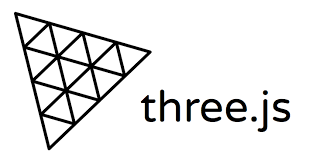
\includegraphics[width=0.25\linewidth]{assets/logos/threeJs.png}
		\label{fig:scrum}
	\end{figure}
\end{itemize}

\subsection{Veille technologique sur les outils de Digital Twin}

Dans le cadre de l’exploration des technologies open-source pour la simulation des opérations aéroportuaires, une veille technologique a été menée, alors plusieurs technologies ont été explorées lors de cette phase, notamment :
\begin{itemize}
	\item \textbf{AnyLogic} : puissant mais propriétaire, avec une courbe d’apprentissage importante.
	\item \textbf{Unity + C\#} : très flexible pour la 3D, mais peu adapté à une intégration web simple.
	\item \textbf{CesiumJS} : excellent pour la visualisation géospatiale, mais moins orienté opérationnels.
	\item \textbf{Babylon.js} : alternative à Three.js avec de bonnes performances graphiques.
\end{itemize}  
\vspace{0.3cm}

À l’issue de cette veille, la plateforme \textbf{GAMA} a été retenue pour les premiers prototypes. 
\begin{itemize}
	\item \textbf{GAMA} : plateforme open-source puissante pour la modélisation multi-agents, utilisée initialement pour deux scénarios de simulation de gestion de stands. 
	\begin{figure}[H]
		\centering
		
\includegraphics[width=0.13\linewidth]{assets/logos/gama.png}
		\label{fig:scrum}
	\end{figure}
	Deux scénarios de simulation ont ainsi été développés. Toutefois, ses limitations en matière d’intégration avec des interfaces front-end web ont conduit à un réajustement technologique.
	
\end{itemize}

\subsection{Comparaison des outils de Digital Twin}

Le tableau~\ref{tab:comparaison_dt} présente une comparaison synthétique entre deux outils envisagés pour le développement du jumeau numérique : \textbf{GAMA} et \textbf{Three.js + Angular}.

\begin{table}[H]
	\centering
	\renewcommand{\arraystretch}{1.1}
	\caption{Comparaison entre GAMA et Three.js + Angular}
	\begin{tabular}{lll}
		\toprule
		\textbf{Critère} & \textbf{GAMA} & \textbf{Three.js + Angular} \\
		\midrule
		Nature & Modélisation multi-agents & Visualisation 3D web interactive \\
		Courbe d’apprentissage & Modérée à élevée & Moyenne (si base en JS/TS) \\
		Intégration front-end & Limitée & Excellente \\
		Interopérabilité avec API & Faible & Haute (via services REST) \\
		Personnalisation graphique & Basique & Avancée (textures, caméras, lumière) \\
		Conclusion & Bon pour les prototypes & Choisi pour le rendu final \\
		\bottomrule
	\end{tabular}
	\label{tab:comparaison_dt}
\end{table}

La combinaison \textbf{Three.js + Angular} a finalement été retenue pour sa capacité à offrir une visualisation 3D web interactive, fluide, et facilement intégrable dans l’interface utilisateur du système final.


\vspace{0.5cm}


\section{Conclusion}
Ce chapitre a présenté la conception fonctionnelle et technique de notre solution, en partant de l’analyse des besoins jusqu’au choix des technologies. Nous avons détaillé l’architecture globale du système ainsi que celle du module d’intelligence artificielle. Une étude comparative des outils de Digital Twin a également permis de justifier les choix technologiques retenus.

Le chapitre suivant portera sur les données utilisées dans notre projet, en décrivant leur source, leur structure, ainsi que les étapes d’analyse et de préparation nécessaires à l'entraînement du modèle.